\documentclass[spanish,notitlepage,letterpaper,12pt]{article} 
\usepackage[spanish]{babel} 
\usepackage{amsmath}
\usepackage{amsfonts}
\usepackage{amssymb}
\usepackage{graphicx}
\usepackage{geometry}      
\geometry{letterpaper}                  
\usepackage{epstopdf}
\usepackage{fancyhdr} % Paquete para encabezados y pies de página
\usepackage{listings}
\usepackage{color}
\usepackage[colorlinks=true,linkcolor=blue,urlcolor=blue]{hyperref}

% Definición de colores para listings
\definecolor{dkgreen}{rgb}{0,0.6,0}
\definecolor{gray}{rgb}{0.5,0.5,0.5}
\definecolor{mauve}{rgb}{0.58,0,0.82}

% Configuración de listings para código Java
\lstset{
  frame=shadowbox,
  language=Java,
  aboveskip=3mm,
  belowskip=3mm,
  showstringspaces=false,
  columns=flexible,
  basicstyle={\small\ttfamily},
  numbers=left,
  numberstyle=\tiny\color{gray},
  keywordstyle=\color{blue},
  commentstyle=\color{dkgreen},
  stringstyle=\color{mauve},
  breaklines=true,
  breakatwhitespace=true,
  tabsize=3,
  rulesepcolor=\color{blue}
}

% Estilo de página para portada/inicio
\fancypagestyle{inicio}{
  \fancyhf{}
  \chead{\bfseries Taller 1 - Grupo C1}
  \rhead{6 de septiembre de 2025}
  \lfoot{\it Diego Chamarraví}
  \cfoot{Universidad Industrial de Santander}
  \rfoot{\thepage}
  \renewcommand{\headrulewidth}{0.5pt}
  \renewcommand{\footrulewidth}{0.5pt}
}

% Estilo de página simple para contenido
\fancypagestyle{simple}{
  \fancyhf{}
  \rhead{6 de septiembre de 2025}
  \rfoot{\thepage}
  \renewcommand{\headrulewidth}{0.5pt}
  \renewcommand{\footrulewidth}{0.5pt}
}

% Márgenes y dimensiones
\voffset = -0.25in
\textheight = 8.0in
\textwidth = 6.5in
\oddsidemargin = 0.in
\headheight = 20pt
\headwidth = 6.5in

\begin{document}

% Portada
\title{
  \textbf{Estructura de datos y análisis de algoritmos \\ Taller 1 Grupo C1} \\
  Introducción a las \textbf{estructuras} de datos y Recursividad.
}
\author{\textbf{Diego Chamarraví}}
\date{6 de septiembre de 2025}

\vspace{50pt}

\maketitle
\thispagestyle{inicio} % portada usa estilo inicio

% Tabla de contenidos
\tableofcontents
\newpage
\thispagestyle{inicio} % tabla de contenidos también usa estilo inicio

% A partir de aquí, cambia el estilo a simple
\pagestyle{simple} 

\section{SOBRE INTRODUCCIÓN A LAS ESTRUCTURAS DE DATOS}

\subsection{Manejo y comprensión de los principios de POO:}

Ejecución del código:

\begin{center}
    \textbf{Primera parte de la ejecución}
    
    \vspace{0.5em}

    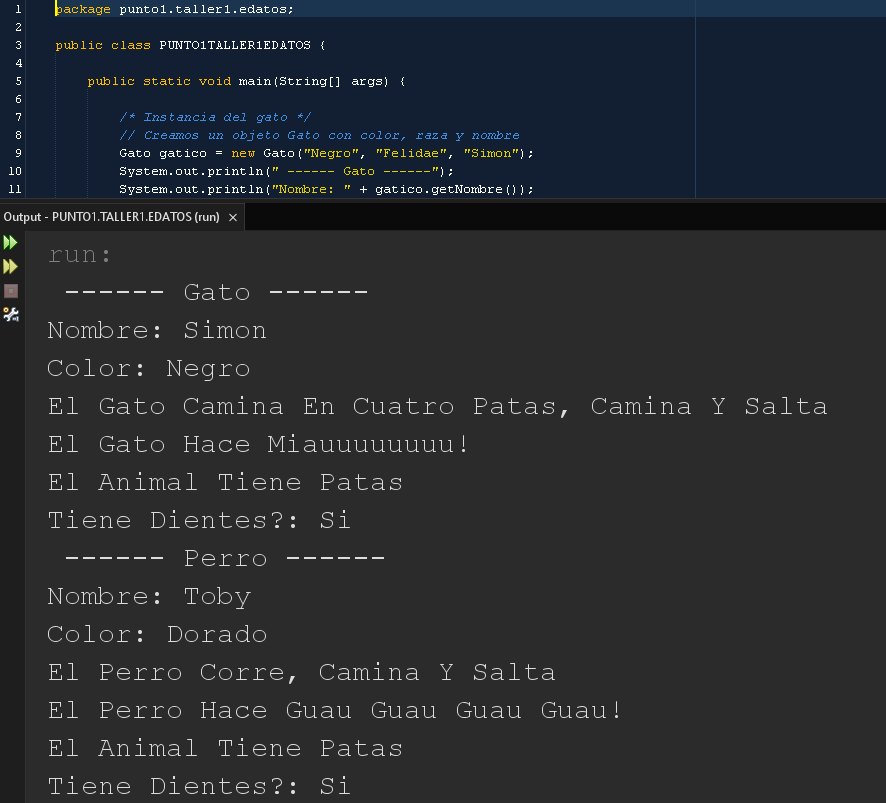
\includegraphics[width=0.8\textwidth]{Figures/1EJECU.png}
\end{center}

\newpage

\begin{center}
    \textbf{Segunda parte de la ejecución}
    
    \vspace{0.5em}

    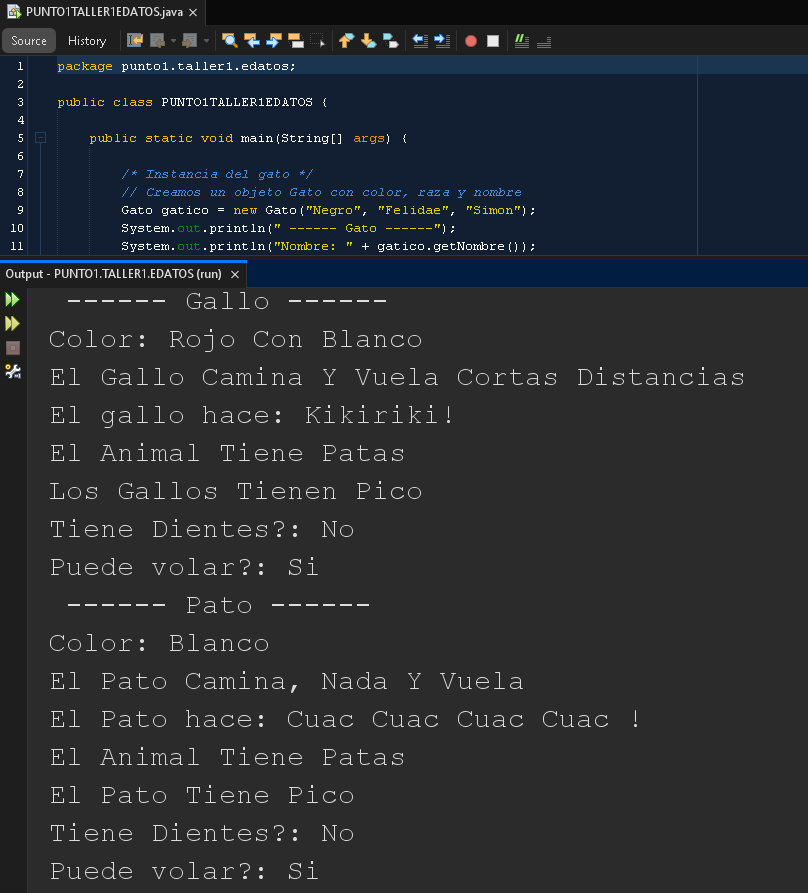
\includegraphics[width=0.8\textwidth]{Figures/2EJECU.png}
\end{center}

\newpage

\begin{center}
    \textbf{Tercera parte de la ejecución}
    
    \vspace{0.5em}

    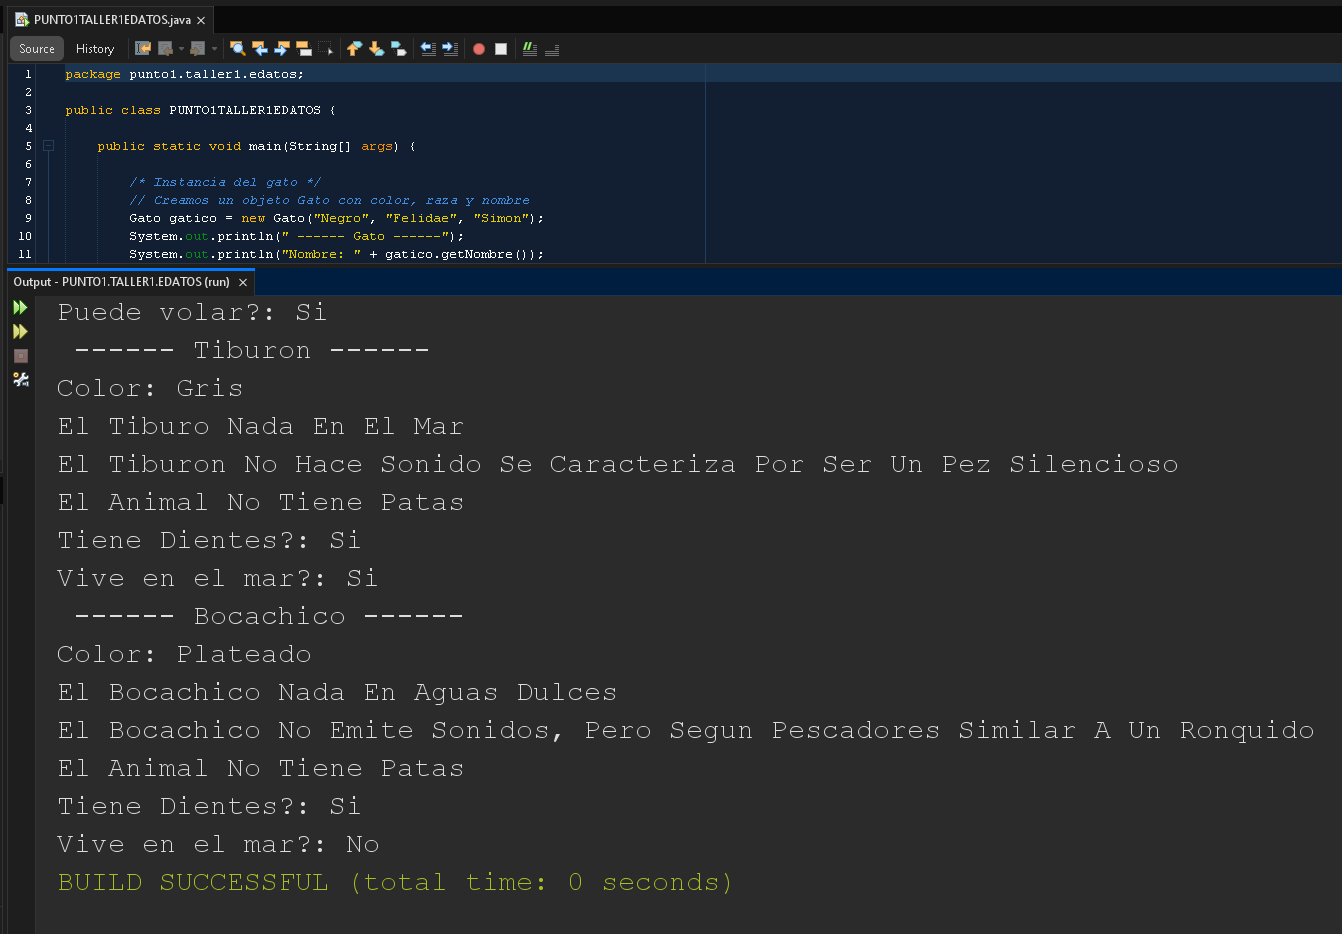
\includegraphics[width=0.8\textwidth]{Figures/3EJECU.png}
\end{center}

\vspace{1em}

\noindent
\textbf{LINKS:} \\
\href{https://github.com/DIEGOVLOGS117/PUNTO1TALLER1EDATOS/tree/master}{Repositorio} \quad | \quad
\href{https://github.com/DIEGOVLOGS117/PUNTO1TALLER1EDATOS/tree/master/UML%20DEL%20PUNTO%201%20TALLER%201%20EDA%20DIEGO%20CHAMARRAV%C3%8D}{UML}

\vspace{1em}

\newpage

\begin{center}
    \textbf{Diagrama UML}
    
    \vspace{0.5em}

    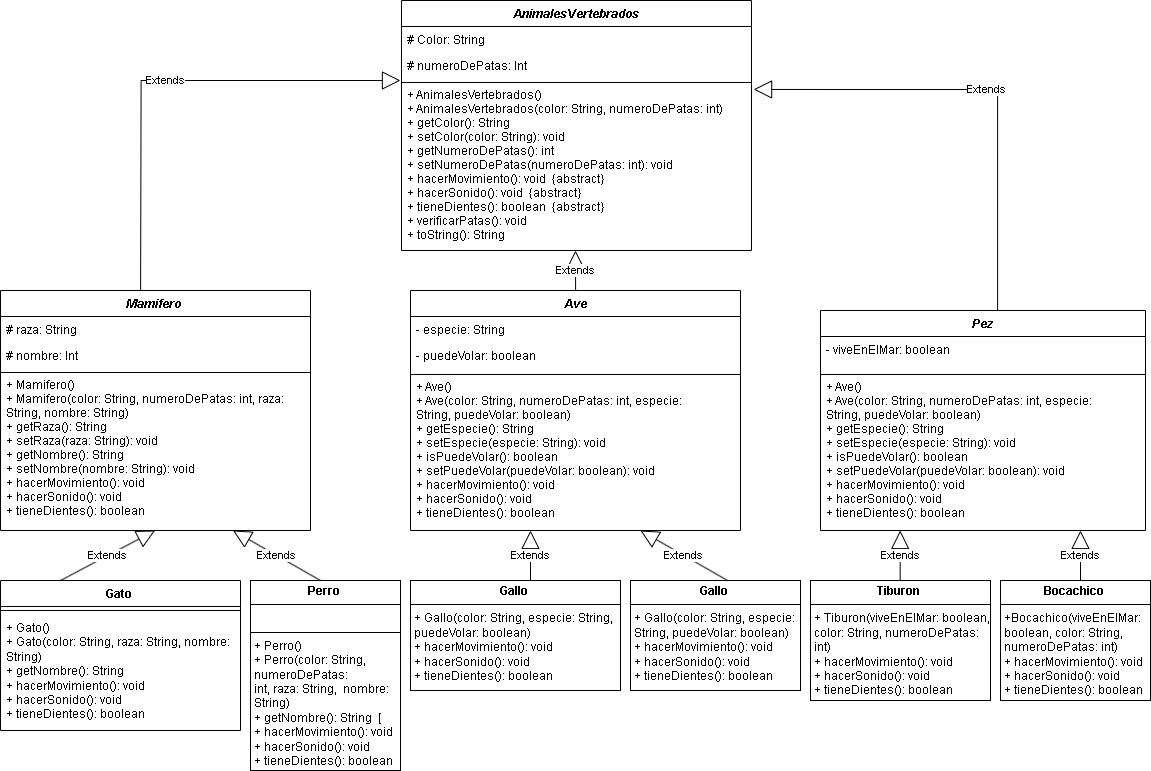
\includegraphics[width=1\textwidth]{Figures/TALLER 1 PUNTO 1 EDA.png}
\end{center}

\vspace{1em}

\vspace{1em}

\newpage

\subsection{Crear una función que ordene un vector de tamaño fijo de manera ascendente o descendente usando la clase Arrays.}

Primera parte orden números:

\begin{lstlisting}[language=Java]
package ordenarnumeros;

public class OrdenarNumeros {

    public static int[] ordenarNumeros(int[] vector, String tipoOrden) {
        int[] resultado = new int[vector.length];
        for (int i = 0; i < vector.length; i++) {
            resultado[i] = vector[i];
        }

        if (tipoOrden == null || 
            (!tipoOrden.equalsIgnoreCase("ascendente") && !tipoOrden.equalsIgnoreCase("descendente"))) {
            System.out.println("El tipo de orden no es válido. Use 'ascendente' o 'descendente'.");
            return resultado;
        }

        boolean swapped;
        int n = resultado.length;

        if (tipoOrden.equalsIgnoreCase("ascendente")) {
            do {
                swapped = false;
                for (int i = 0; i < n - 1; i++) {
                    if (resultado[i] > resultado[i + 1]) {
                        int temp = resultado[i];
                        resultado[i] = resultado[i + 1];
                        resultado[i + 1] = temp;
                        swapped = true;
                    }
                }
                n--;
            } while (swapped);
        } else {
            do {
                swapped = false;
                for (int i = 0; i < n - 1; i++) {
                    if (resultado[i] < resultado[i + 1]) {
                        int temp = resultado[i];
                        resultado[i] = resultado[i + 1];
                        resultado[i + 1] = temp;
                        swapped = true;
                    }
                }
                n--;
            } while (swapped);
        }

        return resultado;
    }

    public static void main(String[] args) {
        int[] numeros = {5, 3, 8, 1, 9};

        int[] asc = ordenarNumeros(numeros, "ascendente");
        int[] desc = ordenarNumeros(numeros, "descendente");

        System.out.print("Números ascendente: ");
        for (int num : asc) {
            System.out.print(num + " ");
        }
        System.out.println();

        System.out.print("Números descendente: ");
        for (int num : desc) {
            System.out.print(num + " ");
        }
        System.out.println();
    }
}
\end{lstlisting}

\newpage

Ejecución del codigo número 1:

\begin{center}
    \textbf{Ejecución 1}
    
    \vspace{0.5em}

    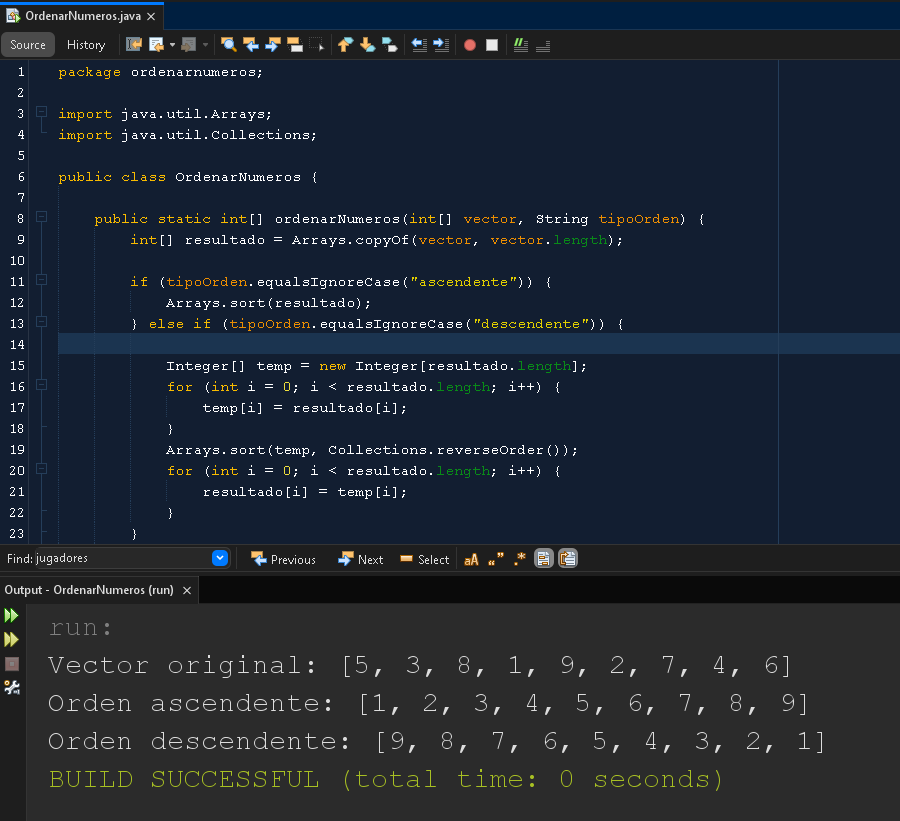
\includegraphics[width=1\textwidth]{Figures/nmeritos.png}
\end{center}

\vspace{0.5 em}

\begin{lstlisting}[caption={Ordenamiento de strings }] [language=Java]
package ordenarnumeros;

import java.util.Arrays;
import java.util.Collections;

public class OrdenarNumeros {

    public static int[] ordenarNumeros(int[] vector, String tipoOrden) {
        int[] resultado = Arrays.copyOf(vector, vector.length);
        
        if (tipoOrden.equalsIgnoreCase("ascendente")) {
            Arrays.sort(resultado);
        } else if (tipoOrden.equalsIgnoreCase("descendente")) {
            
            Integer[] temp = new Integer[resultado.length];
            for (int i = 0; i < resultado.length; i++) {
                temp[i] = resultado[i];
            }
            Arrays.sort(temp, Collections.reverseOrder());
            for (int i = 0; i < resultado.length; i++) {
                resultado[i] = temp[i];
            }
        }
        
        return resultado;
    }

    public static void main(String[] args) {
        int[] numeros = {5, 3, 8, 1, 9, 2, 7, 4, 6};
        
        System.out.println("Vector original: " + Arrays.toString(numeros));
        
        int[] asc = ordenarNumeros(numeros, "ascendente");
        System.out.println("Orden ascendente: " + Arrays.toString(asc));
        
        int[] desc = ordenarNumeros(numeros, "descendente");
        System.out.println("Orden descendente: " + Arrays.toString(desc));
    }
}
\end{lstlisting}

\newpage

Ejecución del codigo número 2:

\begin{center}
    \textbf{Ejecución 2}
    
    \vspace{0.5em}

    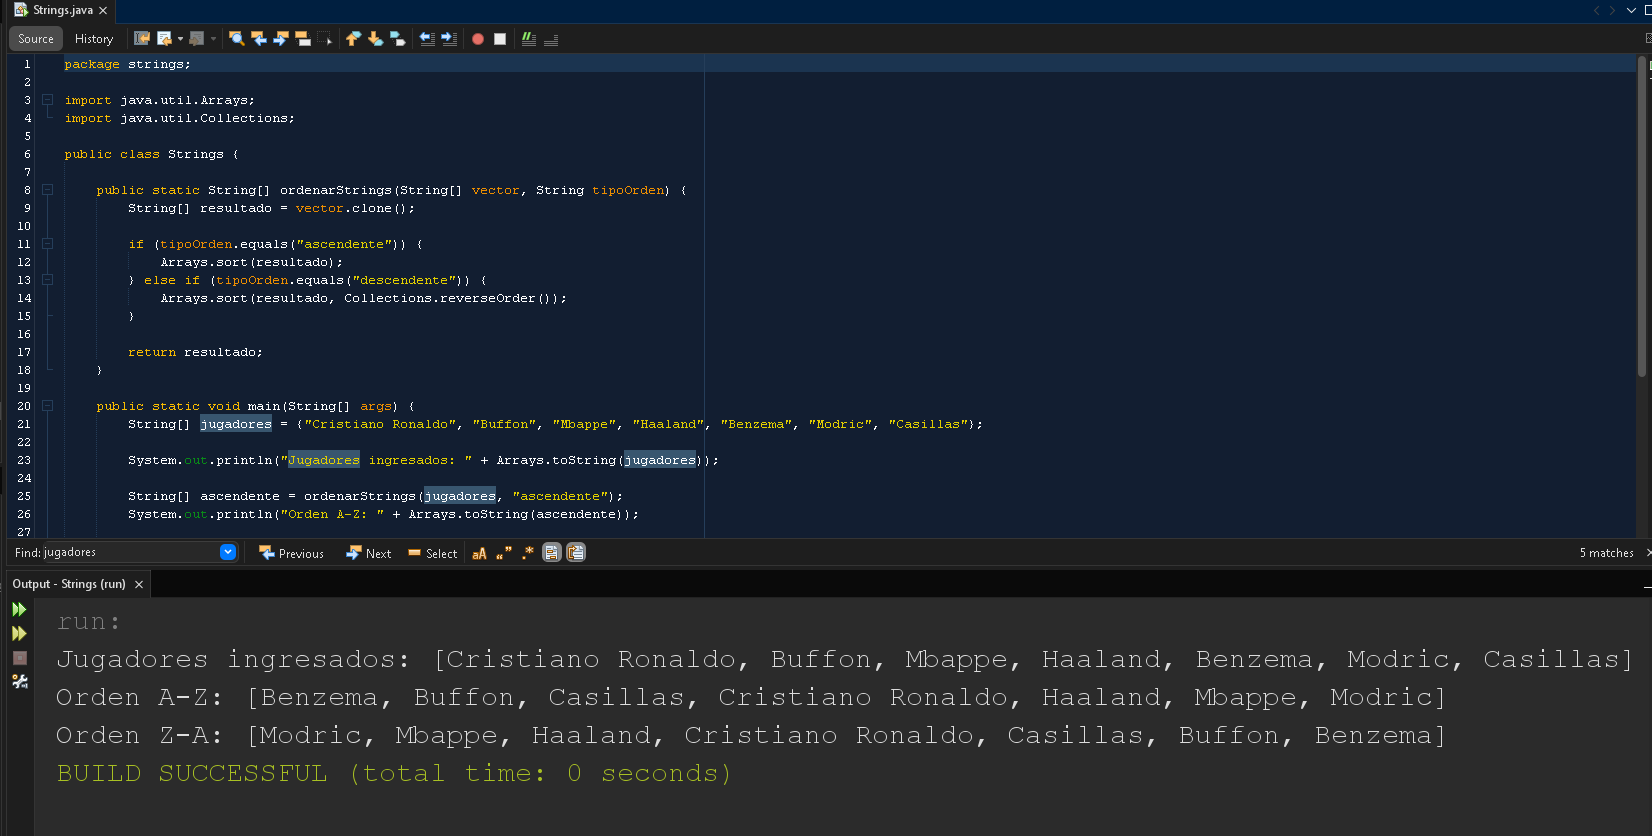
\includegraphics[width=1\textwidth]{Figures/cr7.png}
\end{center}


\subsection{Se busca diseñar un programa que reciba notas de estudiantes}

La respuesta correcta es la opcion 

\subsection{¿Cuáles de las siguientes declaraciones son verdaderas sobre la herencia en Java?}

La respuesta correcta es la d (2, 3 y 4) porque, primeramente, métodos private no se pueden sobreescribir en las subclases, ya que no son visibles afuera de su clase. ¡Comprendes?

Esto quiere decir que no se puede poner la anotación @Override, además su comportamiento se asemeja al de los métodos final, porque tampoco pueden ser cambiados en las clases hijas. Sin dudar, las afirmaciones 2 y 3 son verdaderas. 

Segundamente, el modificador protected da acceso a los miembros dentro del mismo paquete y también a las subclases, aún si están en paquetes diferentes. Eso sugiere que los métodos o atributos protected si se puede acceder en esas subclases, lo cual confirma la verdad de la afirmación 4.

Finalmente, aunque los métodos protected tiene un nivel de acceso especial, no son final por defecto, eso significa que si, que pueden ser sobreescritos en las subclases, por tanto la afirmación 1 es falsa.

\section{SOBRE RECURSIVIDAD}

\subsection{Reemplace \texttt{//Write your code here} en el siguiente código}

\begin{lstlisting}[language=Java]
package recursion;

public class Recursion {
    public static void main(String[] args) {
        System.out.println(encontrarSuma(7));
    }

    public static int encontrarSuma(int n) {

\begin{center}
    \textbf{Ejecución}

    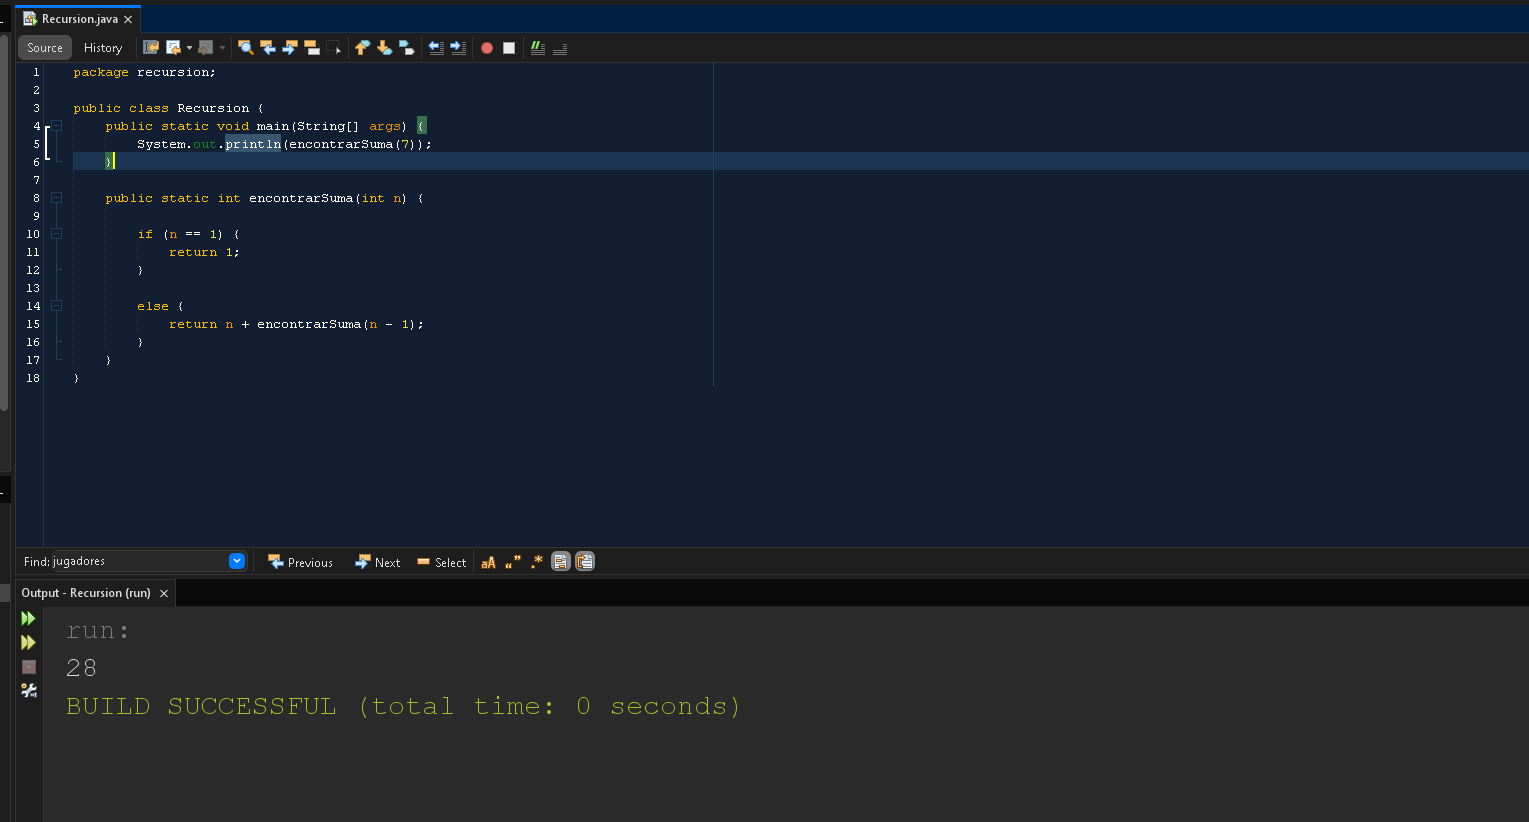
\includegraphics[width=0.9\textwidth]{Figures/image.png}
\end{center}


        if (n == 1) {
            return 1;
        }

        else {
            return n + encontrarSuma(n - 1);
        }
    }
}
\end{lstlisting}

\begin{center}
    \textbf{Ejecución}

    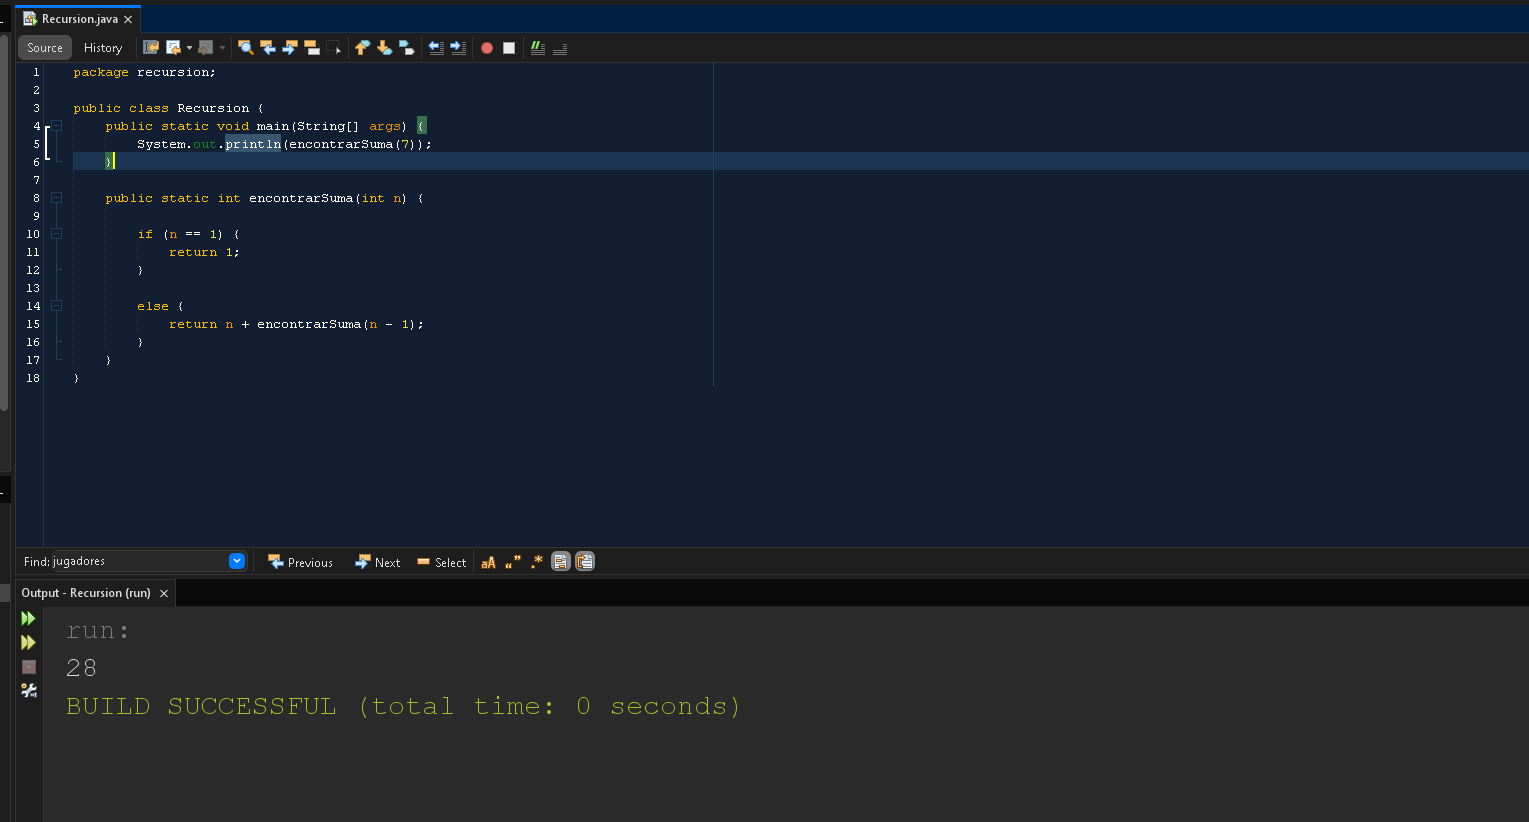
\includegraphics[width=0.9\textwidth]{Figures/image.png}
\end{center}


\subsection{¿Qué hace el siguiente método recursivo? ¿Cuál es la recursión que resuelve?}

El método recursivo hacer(int a, int b) calcula la multiplicación de a por b (es decir, a * b) mediante sumas repetidas de a, b veces.

Caso base: Cuando b == 0, retorna 0 (ya que todo número multiplicado por cero es cero).

Caso recursivo: Retorna a + hacer(a, b-1), lo que suma a al resultado de la llamada recursiva con b-1.

Esto equivale a sumar a consigo mismo b veces, resolviendo así la operación a * b de forma recursiva.

\subsection{Fibonacci optimizado:}

\begin{lstlisting}[language=Java, caption={Fibonacci optimizado}]
package fibo;

public class Fibo {

    public static int fibonacciOptimizado(int n, int[] memo) {
        if (memo[n] != -1) {
            return memo[n];
        }

        if (n == 0) {
            memo[0] = 0;
        } else if (n == 1) {
            memo[1] = 1;
        } else {
            memo[n] = fibonacciOptimizado(n - 1, memo) + fibonacciOptimizado(n - 2, memo);
        }

        return memo[n];
    }

    public static void main(String[] args) {
        int n = 10;
        int[] memo = new int[n + 1];

        for (int i = 0; i <= n; i++) {
            memo[i] = -1;
        }

        fibonacciOptimizado(n, memo);

        System.out.print("Vector de Fibonacci: [");
        for (int i = 0; i <= n; i++) {
            System.out.print(memo[i]);
            if (i < n) {
                System.out.print(", ");
            }
        }
        System.out.println("]");
    }
}
\end{lstlisting}

\begin{center}
    \textbf{Ejecución}

    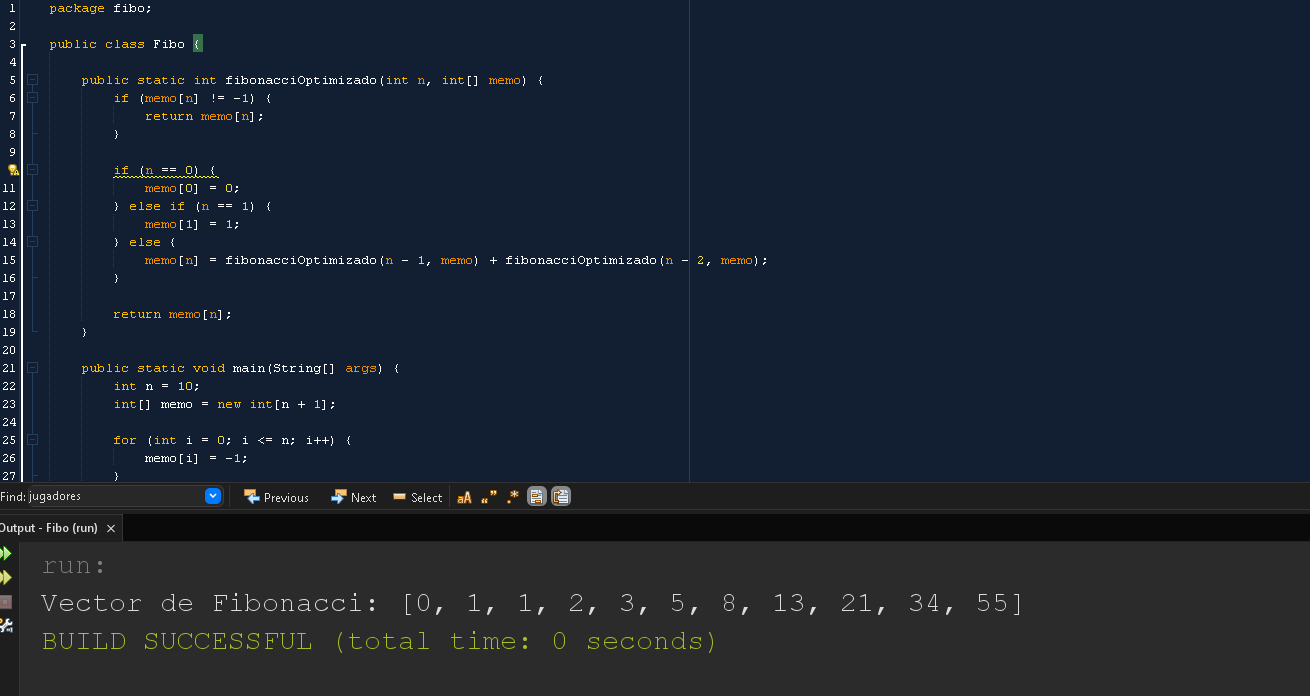
\includegraphics[width=0.9\textwidth]{Figures/Captura de pantalla 2025-09-06 195650.png}
\end{center}



\end{document}